\documentclass[12pt]{article}
\usepackage[spanish]{babel}
\usepackage[utf8]{inputenc}
\usepackage{csquotes}

% Interlineado 1.5
\usepackage{setspace}
\onehalfspacing

% Fuente Times New Roman
\usepackage{mathptmx}

% Acomodar margenes del documento
\usepackage[a4paper, margin=2cm, top=3cm, headheight=50pt]{geometry}

% Paquetes comunes
\usepackage{graphicx, float}
\usepackage{amsfonts, amssymb, amsmath}
\usepackage{physics}
\usepackage{enumerate}
\usepackage[colorlinks=true, citecolor=blue]{hyperref}

% Para graficar
\usepackage{pgfplots}
\usepackage{tikz, color}
\usepackage{tikz-3dplot}
\pgfplotsset{width=15cm, compat=1.12}

% Para automatas
\usetikzlibrary{automata, positioning, arrows, calc}
\tikzset{
        ->,  % makes the edges directed
        >=stealth, % makes the arrow heads bold
        shorten >=2pt, shorten <=2pt, % shorten the arrow
        node distance=3cm, % specifies the minimum distance between two nodes. Change if n
        every state/.style={draw=blue!55,very thick,fill=blue!20}, % sets the properties for each ’state’ n
        initial text=$ $, % sets the text that appears on the start arrow
}

% Encabezados
\usepackage{fancyhdr}
\pagestyle{fancy}
\fancyhf{}
\fancyfoot[C]{\thepage}
\fancyhead[L]{
  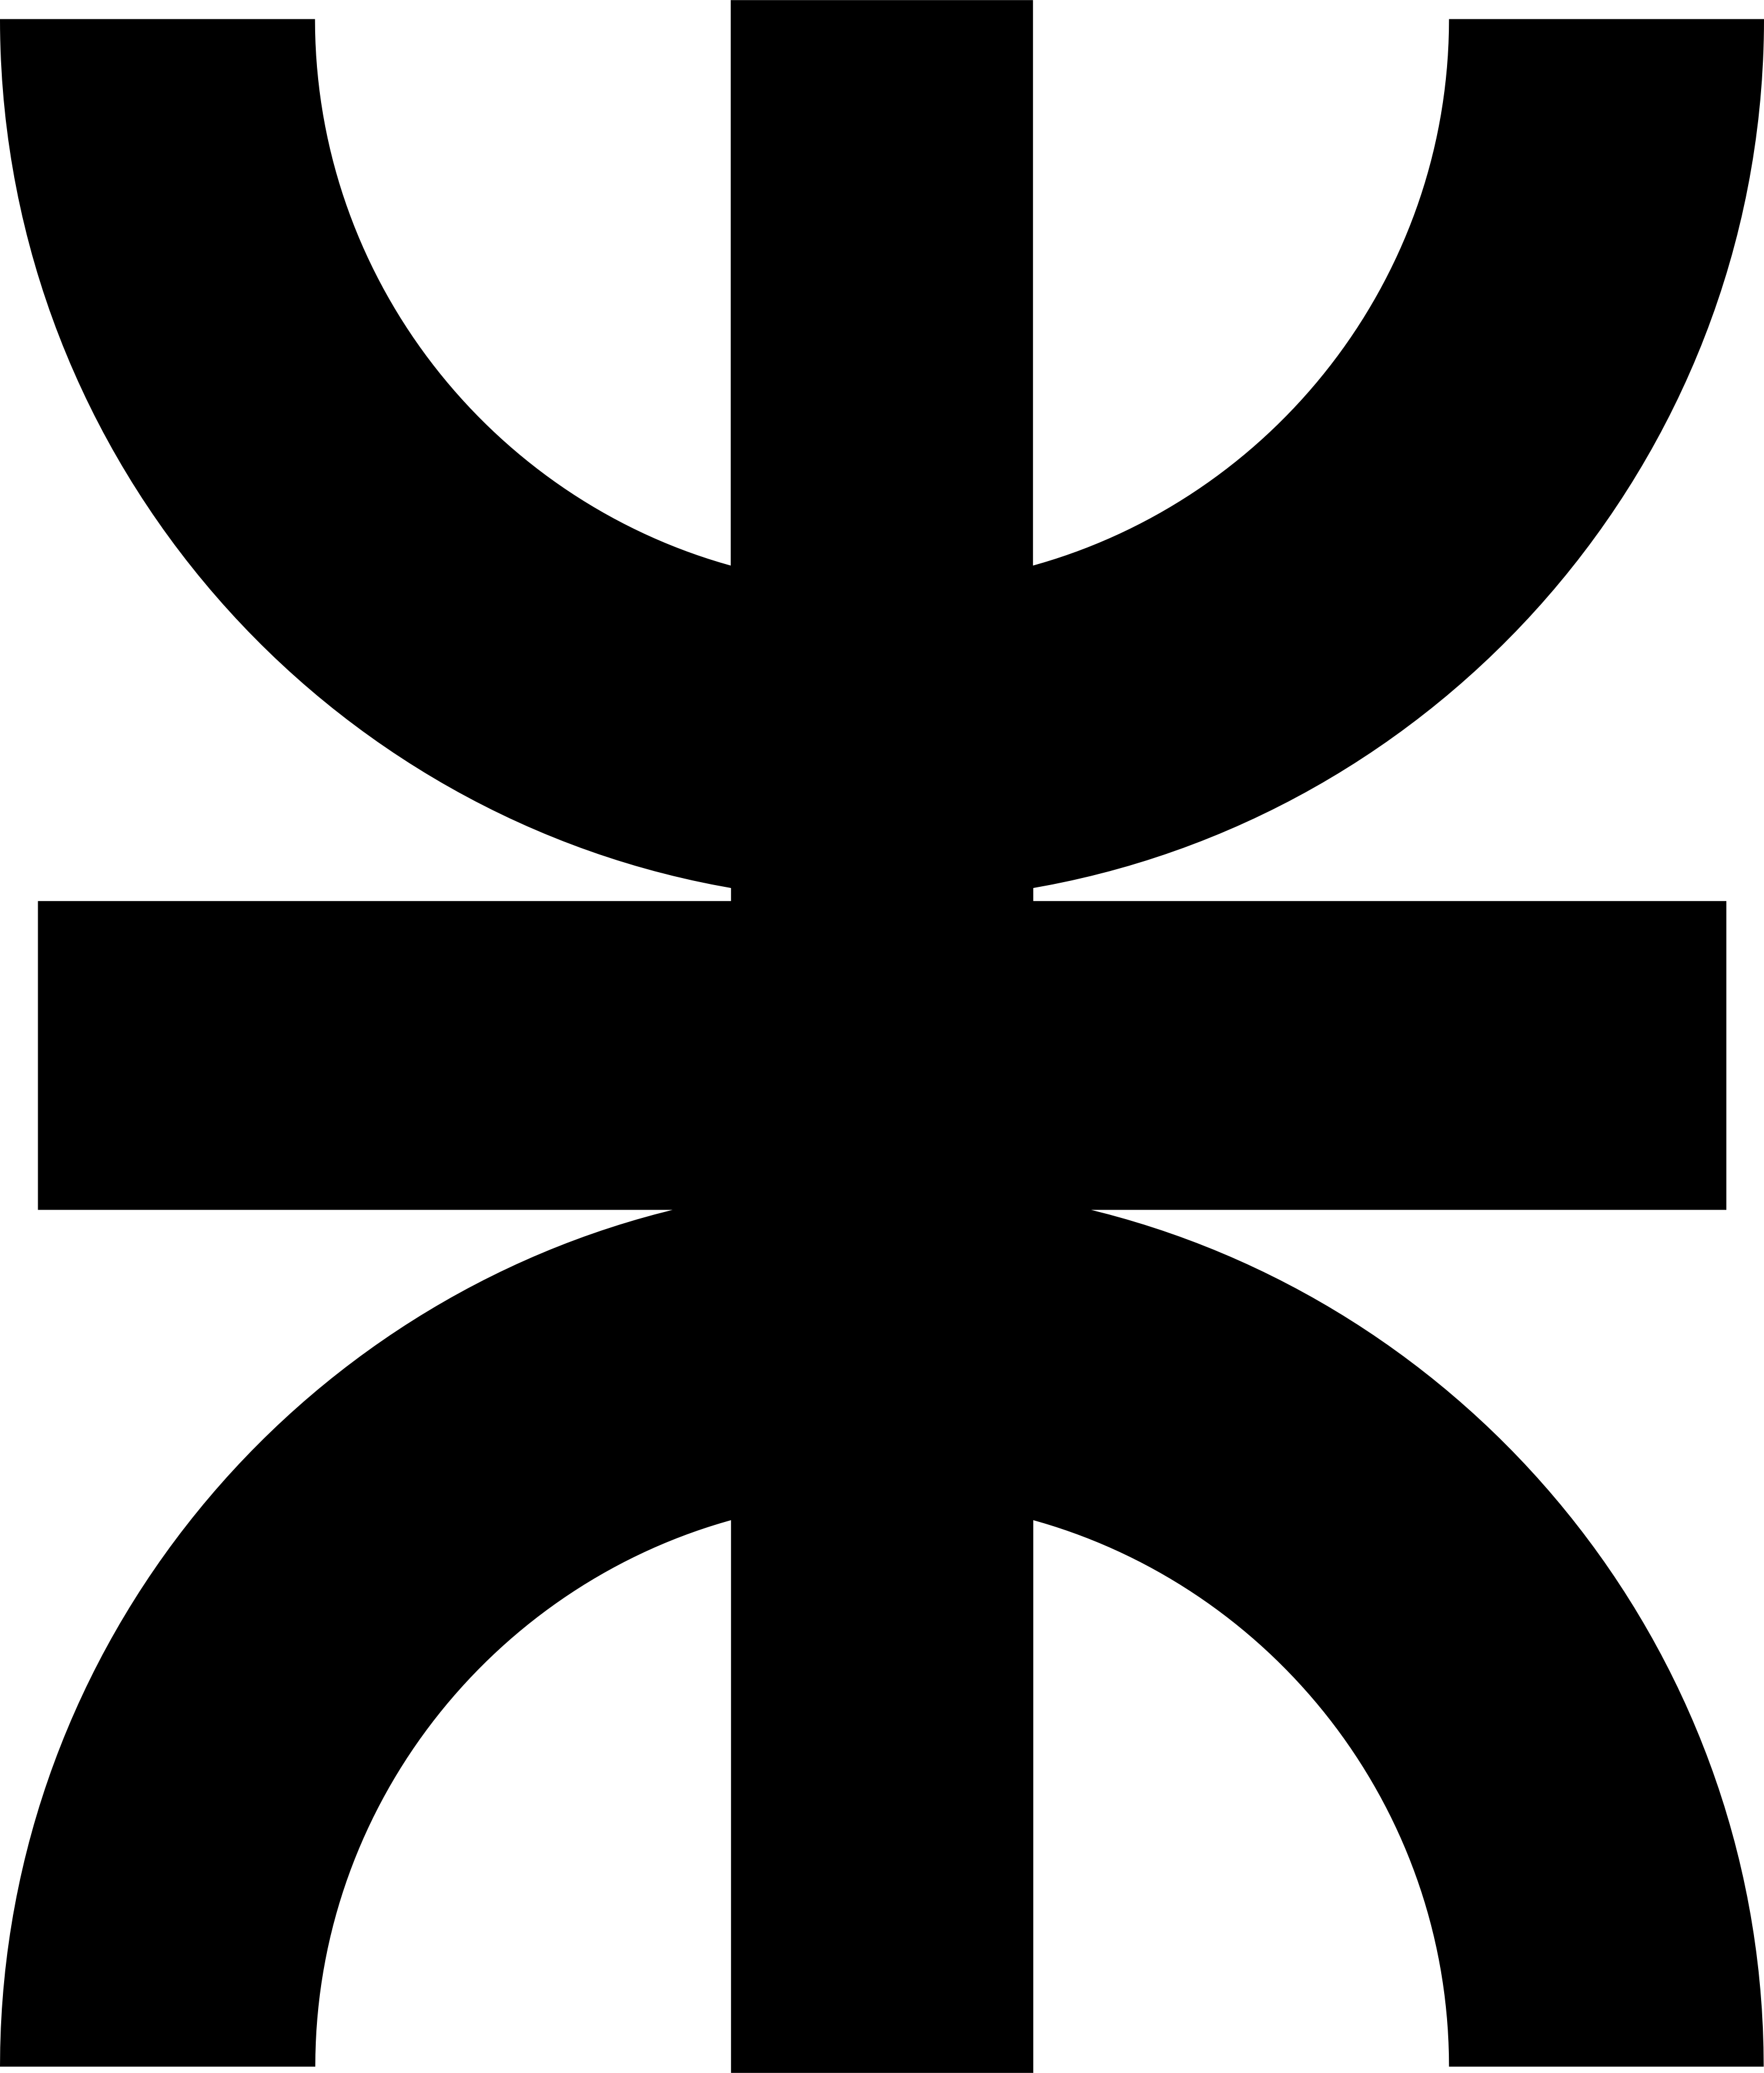
\includegraphics[height=1.2cm]{~/imagenes/logo_utn.png}
  \shortstack[l]{
    {\footnotesize Universidad Tecnológica Nacional} \\
    {\footnotesize Facultad Regional Córdoba} \\
    {\footnotesize Extensión Áulica Bariloche}
  }
}
\fancyhead[C]{
  \shortstack[c]{
    {\footnotesize Física 2} \\
    {\footnotesize Resumen para el primer parcial} \\
    {\footnotesize }
  }
}
\fancyhead[R]{
  \shortstack[r]{
    {\footnotesize Profesor: Santiago Ibañez} \\
    {\footnotesize Alumno: Ricardo Nicolás Freccero} \\
    {\footnotesize Fecha: 10/05/2025}
  }
}

% Para bibliografía
%\usepackage[backend=biber, style=apa]{biblatex}
%\addbibresource{bibliografia.bib}

\begin{document}
\newgeometry{margin=2cm, top=1.5cm}
  \begin{titlepage}
    \centering
    
\includegraphics[width=\linewidth]{~/imagenes/logo_utn_frc.jpg}\\

    \textsc{
      \LARGE Universidad Tecnológica Nacional\\
      \Large Facultad Regional Córdoba - Extensión Áulica Bariloche\\
      \large Ingeniería en Sistemas de Información\\
      Año lectivo 2025\\[0.5cm]
    }

    \rule{\linewidth}{1.0mm}\\[0.4cm]
    \Huge
    \textbf{Fisica 2}\\
    Resumen para el primer parcial\\[0.2cm]
    \LARGE
    Termodinámica
    \rule{\linewidth}{1.0mm}\\
    \large
    \begin{flushleft}
      Profesor: Santiago Ibañez

      Ayudante: Leandro Guzzardo

      Fecha: 10/05/2025
    \end{flushleft}

    \vfill
    \begin{flushright}
      Alumno: Ricardo Nicolás Freccero  

      Número de legajo: 415753
    \end{flushright}
  \end{titlepage}
  
  \restoregeometry
  \tableofcontents
  \newpage

  \section{Temperatura y calor}
  \subsection{Temperatura y equilibrio térmico}
  Los cuerpos que se sienten calientes suelen tener una \textbf{temperatura} más alta que un cuerpo similar que se siente frío. Sin embargo, esta definición es bastante vaga y los sentidos pueden engañarse.

  Para usar la temperatura como medida de calidez necesitamos construir una escala de temperatura. Para esa escala podemos usar cualquier propiedad que podamos medir y que sepamos que varía frente al cambio de temperatura. Por ejemplo, existen los termómetros de mercurio, que es un metal que a temperatura ambiente se encuentra en estado líquido, y al aumentar su temperatura, aumenta su volumen. Otro ejemplo puede ser la presión medida por un manómetro al aumentar o disminuir la temperatura de un gas encerrado en un recipiente de volumen constante. Estas propiedades (volumen y presión) nos dan un número $ (v,p) $ que varía con la calidez y la frialdad, así que pueden usarse para hacer un \textbf{termómetro}.

  Para medir la temperatura de un cuerpo ponemos el termómetro en contacto con él, de manera que se produzca un intercambio de calor entre ambos. Si medimos la temperatura de una taza de café caliente, la taza se va a enfriar un poco y el termómetro se va a calentar hasta que ambos estén a la misma temperatura y ya no varíe la temperatura de ninguno de los dos. En ese momento podemos leer la temperatura del termómetro. Ese estado de equilibrio se llama \textbf{equilibrio térmico}.

  Si dos sistemas están separados por un material \textbf{aislante}, se afectan mutuamente con más lentitud. Un \textit{aislante ideal} es un material que no permite la interacción entre los dos sistemas.

  \subsection{Ley cero de la termodinámica}
  Dados tres sistemas $ A,B,C $ que inicialmente no están en equilibrío térmico. Si separamos $ A $ y $ B $ con una pared aislante ideal, pero dejamos que $ C $ interactúe tanto con $ A $ como con $ B $, al llegar $ A $ y $ C $ al equilibrio térmico y $ B $ y $ C $ al equilibrio térmico, entonces $ A $ y $ B $ se encontrarán en equilibrio térmico también.


  \subsection{Termómetros y escalas de temperatura}
  Existen varias escalas para medir la temperatura de un sistema:
  \begin{itemize}
    \item \textbf{Escala Celsius (°C)}: En la escala Celsius, los cero grados corresponden a la temperatura de congelación del agua con una presión de una atmósfera, y los cien grados marcan el punto de ebullición del agua a la misma presión.


    \item \textbf{Escala Farenheit (°F)}: La temperatura de congelación del agua es 32 °F y la de ebullición es de 212 °F a una presión de una atmósfera.

    \item \textbf{Escala Kelvin (°K)}: Para entender la escala Kelvin conviene saber cómo surgió. La idea era conseguir una escala que no dependa de las propiedades de ningún material para tener una escala absoluta. Se hicieron entonces experimentos con un \textit{termómetro de gas}, que es el termómetro que más se acerca al ideal y se observó lo siguiente.

      El principio de un termómetro de gas muestra que la presión de un gas a volumen constante aumenta con la termperatura. Lo que se hizo entonces fue medir la presión de distintos gases a 0 °C y 100 °C de manera que para cada gas se podían graficar dos puntos en un eje de $ (temperatura, presion) $, y unirlos con una linea. Se encontró así que todos los gases probados tenían rectas diferentes, pero todas convergían en una temperatura hipotética de -273.15 °C, en la que la presión absoluta del gas sería cero. 

      En la escala Kelvin, los 0 °K equivalen a -273.15 °C, y 273.15 °K son equivalentes a 0 °C.
  \end{itemize}

  \begin{figure}[H]
    \centering
    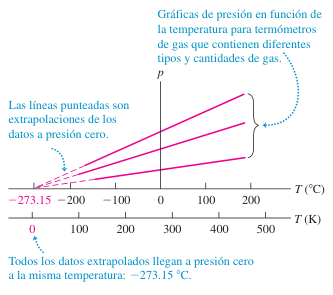
\includegraphics[width=0.5\linewidth]{imagenes/escala-Kelvin.png}
    \caption{Gráfica de presión contra temperatura a volumen constante para gases distintos}
    \label{fig:escala-kelvin}
  \end{figure}
  
  \subsection{Expansión térmica}
  \subsubsection{Expansión lineal}
  Para variaciones de temperaturas que no sean muy grandes (menos de 100 °C), la variación $ \Delta L $ de la longitud de un material es directamente proporcional a la variación $ \Delta T $ de la temperatura del mismo. Se introduce una constante de proporcionalidad $ \alpha $ diferente para cada material y se obtiene la ecuación:
  \[
    \Delta L = \alpha L_{0}\Delta T
  \]
  
  Podemos despejar $ L $ de la ecuación:
  \begin{align*}
    \Delta L &= \alpha L_{0}\Delta T\\
    L - L_{0} &= \alpha L_{0}\Delta T\\
    L &= L_{0} \left(1 + \alpha\Delta T\right)
  \end{align*}

  La constante $ \alpha $, que describe las propiedades des expansión términa de una material dado, se denomina \textbf{coeficiente de expansión lineal}.

  \subsubsection{Expnasión volumétrica}
  Un aumento de temperatura suele aumentar el volumen de materiales. Al igual que en la expansión lineal, la variación del volumen $ \Delta V $ de un material es directamente proporcional al cambio de temperatura $ \Delta T $. En este caso se añade una constante $ \beta $ que se conoce como \textbf{coeficiente de expansión de volumen}.
  \[
    \Delta V  = \beta V_{0}\Delta T
  \]
  
  Para materiales sólidos, hay una relación sencilla entre el coeficiente de expanción de volumen $ \beta $ y  el coeficiente de expansión lineal $ \alpha $. Esta relación se puede deducir considerando un cubo de material con longitud de lado $ L $ y volumen $ V = L^{3} $. Al aumentar la temperatura en $ dT $, la longitud del lado aumenta en $ dL $ y el volumen aumenta en $ dV $ dada por:
  \[
  dV = \frac{dV}{dL}dL = 3L^{2}dL
  \]
  
  Por la ecuación de la expansión lineal, sabemos que $ dL $ es:
  \[
  dL = \alpha L_{0}dT
  \]

  Ahora sustituimios $ L $ por el valor inicial $ L_{0} $ y $ dL $ por lo que obtuvimos recién:
  \[
  dV = 3L_{0}^{2}\alpha L_{0}dT = 3L_{0}^{3}\alpha dT
  \]

  Como $ V_{0} = L_{0}^{3} $, esto implica que $ dV $ también lo podemos expresar como:
  \[
  dV = 3\alpha V_{0}dT
  \]

  Y podemos deducir que $ \beta = 3\alpha $ por la ecuación de la expansión de volumen.
  
  \subsection{Cantidad de calor}
  Si metemos una cuchara fría en una taza con café caliente, la cuchara se calienta y el café se enfría para establecer el equilibrio térmico. Esto se debe a que hay un transferencia de energía de un sistema al otro. La transferencia de energía que se da exclusivamente por una diferencia de temperatura se denomica \textit{flujo de calor} o \textit{transferencia de calor}, y la energía transferencia es lo que llamamos \textbf{calor}.

  \subsubsection{Calor específico}
  Usamos el símbolo $ Q $ para cantidad de calor. cuando el calor está asociado a un cambio de temperatura infinitesimal $ dT $, lo llamamos $ dQ $. L a cantidad de calor $ Q $ necesaria para elevar la temperatura de una mása $ m $ de cierto material de $ T_{1} $ a $ T_{2} $ es aproximadamente proporcional al cambio de temperatura $ \Delta T $ y a la mása $ m $ del material. Cada material requiere distintas cantidades de energía para elevar su temperatura, por lo que a la ecuación se le agrega una constante $ c $ llamada \textbf{calor específico}:
  \[
  Q = mc\Delta T
  \]

  \fbox{\parbox{0.9\linewidth}{
  \textbf{Nota}

  Como el calor es la transferencia de energía a causa de una diferencia de temperatura, no existe la \textit{cantidad de calor de un cuerpo}. No tiene sentido decir eso.
  }}\vspace{0.2cm}

  \subsubsection{Capacidad calorífica molar}
  A veces es más útil describir una cantidad de sustancia en términos del número de moles $ n $, en vez de la mása $ m $ del material. Recordemos que la mása $ m $ de un material y su número de moles están relacionados por la siguiente ecuación $ m = nM $ donde $ M $ es la mása molar. De esta manera podemos sustituir $ m $ en la ecuación del calor:
  \[
  Q = nMc\Delta T
  \]

  El producto $ Mc $ es la \textbf{capacidad calorífica molar} (o \textit{calor específico molar}) y se denota con $ C $. De esta manera, tenemos que:
  \[
  Q = nC\Delta T
  \]

  En sólidos, las mediciones de calor específico se suelen hacer a presión atmosférica constante; los valores correspondientes se llaman \textit{calor específico} y \textit{capacidad calorífica molar a presión constante}, denotados con $ c_{p} $ y $ C_{p} $. En el caso de un gas, es más fácil mantener el volumen constante; los valores correspondientes son \textit{calor específico} y \textit{capacidad calorífica molar a volumen constante}, denotados con $ c_{v} $ y $ C_{v} $ respectivamente. Para una sustancia dada, $ C_{v} $ y $ C_{p} $ son diferentes. Si el sistema puede expandirse al agregar calor, hay un intercambio adicional de energía porque el sistema efectúa \textit{trabajo} sobre su entorno. Si el volumen es constante, el sistema no efectúa trabajo. 

  \subsubsection{Cambios de fase}
  Usamos el término \textbf{fase} para describir un estado específico de la materia, como sólido, líquido o gas. Una transición de una fase a otra es un \textbf{cambio de fase}. Para una presión dada, lso cambios de fase se dana una temperatura definida, generalmente acompañada por absorción o emisión de calor, y un cambio de volumen y densidad.

  Supongamos que tenemos un recipiente con agua líquida a 20 °C y a una presión de 1 atmósfera. Supongamos también que el recipiente está tapado, pero esta tapa se puede mover libremente de manera que al agua dentro puede variar su volumen a presión constante. En estas condiciones, el agua existe en fase líquida y se encuentra en estado de \textbf{líquido comprimido} o \textbf{líquido subenfriado}, lo que significa que \textit{no está a punto de evaporarse}. Si aumentamos la temperatura del agua hasta los 100 °C, el agua permanece líquida, pero cualquier adición de calor hace que se vaporice algo de agua; es decir, está a punto de tener lugar un proceso de cambio de fase de líquido a vapor. En este estado decimos que el agua es un \textbf{líquido saturado}. 

  Una vez que empieza la ebullición, si sigue habiendo una transferencia de calor hacia el agua, el aumento de temperatura se detiene hasta que se evapora todo el líquido. Durante este proceso, el recipiente contiene cantidades de agua líquida y vapor de agua y la temperatura del sistema es de 100 °C. En este estado, el vapor está \textit{a punto de condensarse} y decimos que  se encuentra como \textbf{vapor sautrado}. Pasado este punto, cuando ya toda el agua se evaporó, la temperatura del vapor comienza a elevarse por encima de los 100 °C y decimos que el vapor se encuentra como \textbf{vapor sobrecalentado}.

  \section{Propiedades térmicas de la materia}
  Las condiciones enque existe un material dado se describen con cantidades físicas como presión, volumen, temperatura y cantidad de sustancia. Estas variables describen el \textit{estado} del material y se llaman \textbf{variables de estado}.

  \subsection{La ecuación del gas ideal}
  Las mediciones del comportamiento de diversos gases dan origen a tres conclusiones:
  \begin{enumerate}[1.]
    \item El volumen $ V $ es proporcional al número de moles $ n $.

    \item El columen varía \textit{inversamente} con la presión absoluta $ p $.

    \item La presión es porporcional a la temperatura \textit{absoluta}.
  \end{enumerate}

  Estas tres relaciones se puede combinar en una sola ecuación, llamada \textbf{ecuación del gas ideal}:
  \[
  pV = nRT
  \]

  donde $ R $ es una constante de proporcionalidad. El \textbf{gas ideal} es una gas para el que la ecuación anterior se cumple con precisión a \textit{todas} las presiones y temperaturas. 

  La constante $ R $ es la misma para todos los gases. Su valor numérico depende de las unidades en las que expresamos $ p, V, T $. En unidades del SI, con $ p $ en $ Pa $ ($ 1Pa = 1\frac{N}{m^{2}} $) y $ V $ en $ m^{3} $, el valor de $ R $ es:
  \[
  R = 8.314472\frac{J}{mol.K}
  \]

  \subsection{Graficas pV}
  Las gráficas de la relación $ p $-$ V $-$ T $ en realidad se representan como superficies ya que tenemos tres variables. Sin embargo, podemos usar curvas de nivel para representar las gráficas de forma bidimensional, suele ser más útil. Una de las gráficas bidimensionales más usadas es la \textbf{gráfica pV}, que expresa la presión en fucnión del volumen, en la que cada curva representa el comportamiento del gas a temperatura constante. Dichas curvas se denominan \textbf{isotermas}.

  \begin{figure}[H]
    \centering
    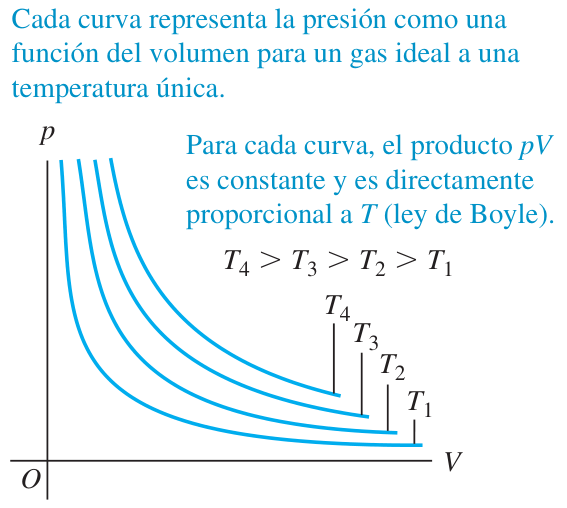
\includegraphics[width=0.5\linewidth]{imagenes/g-pv-gas-ideal.png}
    \caption{Grafica pV para un gas ideal.}
    \label{fig:pv-gas-ideal}
  \end{figure}
  
  \begin{figure}[H]
    \centering
    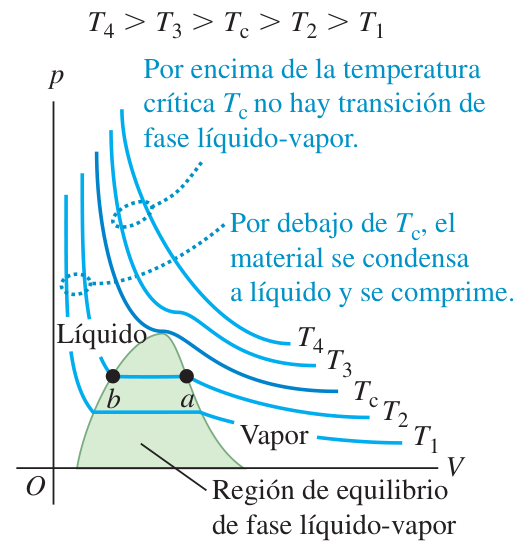
\includegraphics[width=0.5\linewidth]{imagenes/g-pv-gas-no-ideal.png}
    \caption{Gráfica pV para un gas no ideal.}
    \label{fig:pv-gas-no-ideal}
  \end{figure}

  \subsection{Moles y número de Avogadro}
  Un mol es la cantidad de sustancia que contiene tantas moléculas como átomos hay en $ 0.012kg $ de carbono 12.

  El número de moléculas en un mol se denomina número de \textbf{número de Avogadro} y se denota con $ N_{A} $:
  \[
  N_{A} = 6.02214199\times 10^{23}\frac{\text{moléculas}}{\text{mol}}
  \]

  La mása molar $ M $ de un compuesto es la mása de un mol:
  \[
  M = N_{A}m
  \]

  La masa total $ m_{\text{total}} $ de una cantidad dada de un compuesto es el número de moles $ n $ multiplicado por la masa de un mol $ M $
  \[
  m_{\text{total}} = nM
  \]
  
  \subsection{Modelo cinético-molecular del gas ideal}
  La idea es armar un modelo sencillo del gas ideal para poder predecir la capacidad caloríficar molar de un gas ideal.
  Para nuestro \textit{modelo cinético molecular} vamos a suponer lo siguiente:
  \begin{enumerate}[1.]
    \item Un recipiente con volumen $ V $ contiene un número muy grande $ N $ de moléculas idénticas, cada una con mása $ m $.

    \item Las moléculas se comportan como partículas puntuales; su tamaño es pequeño en compración con la distancia media entre pertículas y las dimensiones del recipiente.

    \item Las moléculas están en constante movimiento, y obedecen las leyes del movimiento de Newton. Las  moléculas chocan ocasinalmente con las paredes del recipiente. Tales chocques son perfectamente elásticos.

    \item Las paredes del recipiente son perfectamente rígidas y con más infinita; no se mueven.
  \end{enumerate}

  \subsubsection{Colisiones y presión del gas}
  Durante los choques, las moléculas ejerces fuerzas sobre las paredes del recipiente; éste es el origen de la presión del gas. En el choque representado en la Figura \ref{fig:choque-gas}, la componente de velocidad paralela a la pared no cambia y la componente perpendicular a la pared invierte su dirección sin cambiar de magnitud.

  \begin{figure}[H]
    \centering
    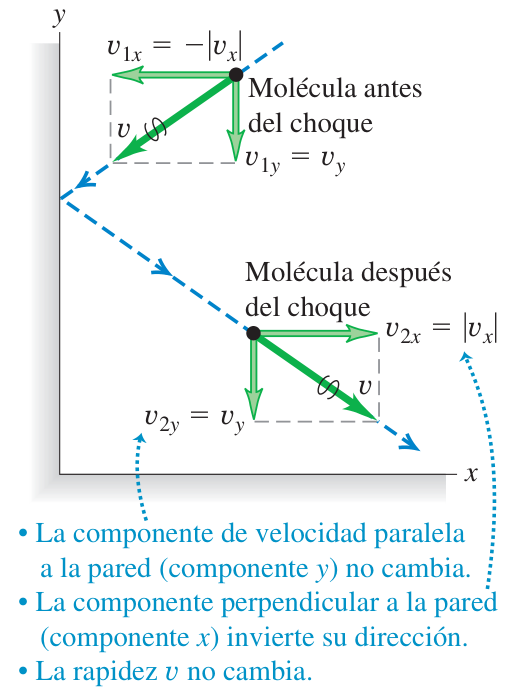
\includegraphics[width=0.5\linewidth]{imagenes/choque-molecula-gas.png}
    \caption{Choque elástico de una molécula con la pared de un recipiente idealizado.}
    \label{fig:choque-gas}
  \end{figure}
  
  Para empezar, supongamos que todas las moléculas del gas tienen la misma \textit{magnitud} de la componente $ x $ de velocidad, $ \left|v_{x}\right| $. Esto no es correcto pero no sirve para entender algunos conceptos básicos.

  En la Figura \ref{fig:choque-gas} vemos que la componente $ x $ de velocidad cambia de $ -\left|v_{x}\right| $ a $ +\left|v_{x}\right| $, así que la variación de la cantidad de movimiento ($ \Delta P = m_{f}v_{f}-m_{0}v_{0} $) en $ x $ es $ m\left|v_{x}\right| - (-m\left|v_{x}\right|) = 2m\left|v_{x}\right| $.

  Si una molécula va a chocar con cierta área $ A $ dentro de un intervalo de tiempo $ dt $, al comenzar ese intervalo $ dt $ la partícula tiene que estar como mucho a una distancia $ \left|v_{x}\right|dt $ de la pared. Entonces, el número de moléculas que chocan con $ A $ durante un intervalo de tiempo $ dt $ es igual al número de moléculas que están dentro de un cilindro con volumen $ A\left|v_{x}\right|dt $ cuya velocidad está dirigida hacia la pared. Si suponemos que las moléculas están esparcidas de manera uniforme, la cantidad de moléculas por unidad de volumen es $ \frac{N}{V} $, y podemos decir que la \textit{cantidad de moléculas de este cilindro} es $ \frac{N}{V}A\left|v_{x}\right|dt $. En promedio, la mitad de las moléculas se están acercando a la pared y la otra mitad se está alejando, así que el número de choques con $ A $ durante $ dt $ es:
  \[
  \frac{1}{2}\frac{N}{V}A\left|v_{x}\right|dt
  \]
  
  Para el sistema de todas las moléculas del gas, la variación total de cantidad de movimiento $ dP_{x} $ durante $ dt $ es la cantidad de movimiento de una partícula multiplicado por la cantidad de partículas que chocan contra la pared.
  \[
  dP_{x} = \left(\frac{1}{2}\frac{N}{V}A\left|v_{x}\right|dt\right)\left(2m\left|v_{x}\right|\right) = \frac{NAmv_{x}^{2}dt}{V}
  \]

  La tasa de cambio de la componente de cantidad de movimiento $ P_{x} $ es:
  \[
  \dv[]{P_{x}}{t} = \frac{NAmv_{x}^{2}}{V}
  \]

  Y ya sabemos que $ F = \dv[]{P}{t} $. También sabemos que la presión es la fuerza ejercida sobre el área, de manera que:
  \[
    p = \frac{F}{A} = \frac{Nmv_{x}^{2}}{V}
  \]

  De todas maneras, sabemos que estamos cometiendo un error al suponer que todas las partículas se mueven a la misma velocidad. En realidad las partículas se mueven en todas las direcciónes de manera que:
  \[
  v^{2} = v_{x}^{2} + v_{y}^{2} + v_{z}^{2}
  \]

  Sin embargo, en nuestro modelo no hay una diferencia real entre las direcciones $ x $, $ y $ y $ z $ ya que las rapideces moleculares son tan altas en un gas típico que los efectos de la gravedad son insignificantes. Se deduce entonces que $ v_{x}^{2} $, $ v_{y}^{2} $ y $ v_{z}^{2} $ son iguales, por lo que $ v_{x}^{2} = \frac{1}{3}v^{2} $.

  La ecuación anterior entonces se convierte en 
  \[
  pV = \frac{1}{3}Nmv^{2} = \frac{2}{3}N\left[\frac{1}{2}mv^{2}\right]
  \]

  Observemos que $ \frac{1}{2}mv^{2} $ es la energía cinética de traslación de una sola molécula del gas. El producto de esto por el número de moléculas $ N $ es igual a la energía cinética total del gas $ K $. 
  \[
  K = N\frac{1}{2}mv^{2}
  \]
  \[
    pV = \frac{2}{3}K
  \]

  Si compararmos esto con la ecuación del gas ideal tenemos que 
  \[
  K = \frac{3}{2}nRT
  \]

  La energía de traslación de una sola molécula es la energía cinética de traslación $ K $ dividido la cantidad de moléculas $ N $
  \[
  \frac{K}{N} = \frac{1}{2}mv^{2} = \frac{3nRT}{2N}
  \]

  El número total de moléculas $ N $ es el número de moles $ n $ multiplicado por el número de Avogadro $ N_{A} $, de manera que
  \[
    N = nN_{A} \quad \frac{n}{N} = \frac{1}{N_{A}}
  \]

  y
  \[
  \frac{K}{N} = \frac{1}{2}mv^{2} = \frac{3}{2}\frac{R}{N_{A}}T
  \]

  La razón $ \frac{R}{N_{A}} $ se llama \textbf{constante de Boltzmann} y se denota con la letra $ k $.

  \subsubsection{Rapideces moleculares}
  A partir de las ecuaciones anteriores podemos obtener expresiones para la raíz cuadrada de $ v^{2} $, llamada \textbf{rapidez eficaz} o \textbf{rapidez rms}
  \[
    v_{rms} = \sqrt[]{v^{2}} = \sqrt[]{\frac{3kT}{m}} = \sqrt[]{\frac{3RT}{M}}
  \]

  \section{Primera ley de la termodinámica}
  \subsection{Sistemas termodinámicos}
  Un \textbf{sistema termodinámico} es cualquier conjunto de objetos que conviene considerar como un aunidad, y que podría intercambiar energía con el entorno. Un proceso en el que se producen cambios en el estado de un sistema termodinámico, se denomina \textbf{proceso termodinámico}.

  \subsubsection{Signos del calor y el trabajo en termodinámica}
  Describimos las relaciones de energía de cualquier proceso temodinámico en términos de la cantidad de calor $ Q $ agregada al sistema y el trabajo $ W $ realizado por él. Ambos pueden ser negativos, positivos o cero. Un valor positivo de $ Q $ representa un flujo de calor \textit{hacia} el sistema (está entrando calor al sistema), con un suministro de energía correspondiente; un $ Q $ negativo representa flujo de calor hacia \textit{afuera} del sistema (sale calor del sistema). Un valor positivo de $ W $ representa el trabajo realizado \textit{por} el sistema contra el entorno (como un gas en expansión), y corresponde a la energía que \textit{sale} del sistema. Un $ W $ negativo, como el realizado durante la compresión de un gas, es cuando el entorno realiza trabajo \textit{sobre} el sistema, y representa energía que \textit{entra} en el sistema.

  \subsection{Trabajo realizado al cambiar el volumen}
  Supongamos que tenemos una cantidad de gas en un cilindro con un pistón móvil. Al expandirse el gas, empuja el pistón realizando un trabajo sobre el mismo.

  \begin{figure}[H]
    \centering
    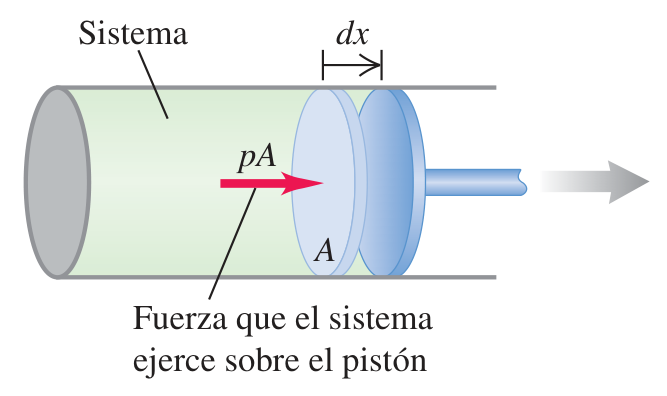
\includegraphics[width=0.5\linewidth]{imagenes/trabajo-gas-piston.png}
    \caption{Cilindro con pistón móvil que contiene gas.}
    \label{fig:gas-piston}
  \end{figure}
  
  En la Figura \ref{fig:gas-piston} vemos un sistema cuyo volumen puede cambiar en un cilindro con pistón móvil. Supongamos que el área transversal del cilindro es $ A $ y la presión ejercida por el sistema en la cara del pistón es $ p $. Recordemos que la fórmula del trabajo es 
  \[
  W = \int_{}^{} F \,dx
  \]

  En este caso, la fuerza es $ F = pA $ y el desplazamiento es $ dx $ de manera que
  \[
    dW = F\,dx = pA\,dx
  \]

  Pero $ A\,dx = dV $, donde $ dV $ es el cambio infinitesimal de volumen del sistema. Así, podemos expresar el trabajo efectuado por el sistema en este cambio infinitesimal de volumen como 
  \[
  dW = p\,dV
  \]

  En un cambio finito de volumen de $ V_{1} $ a $ V_{2} $, tenemos que
  \[
  W = \int_{V_{1}}^{V_{2}} p \,dV
  \]

  \begin{figure}[H]
    \centering
    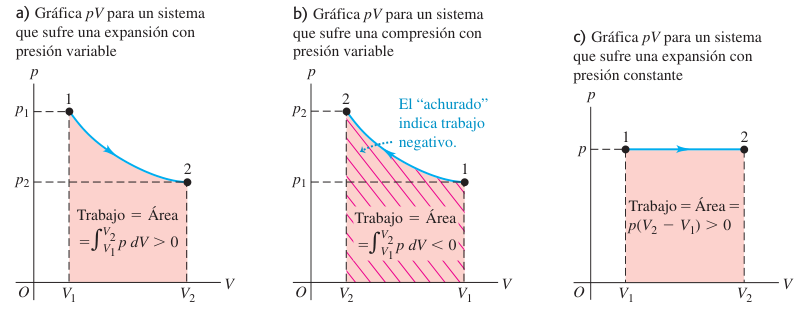
\includegraphics[width=0.7\linewidth]{imagenes/trabajo-g-pv.png}
    \caption{El trabajo efectuado es igual al área bajo la curva en una gráfica pV.}
    \label{fig:trabajo-pv}
  \end{figure}
  
  Vemos que el trabajo es positivo cuando un sistema se expande, y es negativo cuando se comprime. Si la presión $ p $ se mantiene constante mientras el volumen cambia de $ V_{1} $ a $ V_{2} $, el trabajo efectuado por el sistema es $ W = p(V_{2}-V_{1} $.

  \fbox{\parbox{0.9\linewidth}{
  \textbf{Nota}
  
  En cualquier proceso donde el volumen sea constante, el sistema no realiza trabajo porque no hay desplazamiento.
  }}\vspace{0.2cm}

  \subsection{Trayectoria entre estados temodinámicos}
  \subsubsection{Trabajo efectuado en un proceso termodinámico}
  Cuando un sistema cambia de un estado inicial a uno final, pasa por una serie de estados intermedios, a los que llamamos \textbf{trayectoria}. Siempre hay un número infinito de posibilidades para dichos estados intermedios. Si todos son estados de equilibrio, la trayectoria podrá verse en una gráfica $ pV $ (necesitamos que sean de equilibrio porque en la gráfica $ pV $ las curvas representan \textit{isotermas}).

  \begin{figure}[H]
    \centering
    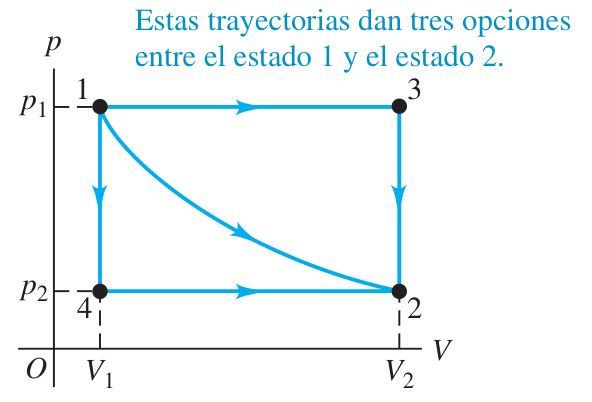
\includegraphics[width=0.5\linewidth]{imagenes/trabajo-trayectoria.png}
    \caption{El trabajo efectuado depende de la trayectoria.}
    \label{fig:trabajo-trayectoria}
  \end{figure}
  
  En la Figura \ref{fig:trabajo-trayectoria} podemos ver que, el punto 1 representa un estado inicial con presión $ p_{1} $ y volumen $ V_{1} $, y el punto 2 representa un estado final $ p_{2} $ y $ V_{2} $. Para pasar del estado 1 al 2, podríamos mantener la presión en $ p_{1} $ mientras el sistema se expande al volumen $ V_{2} $ (punto 3) y luego reducir la presión a $ p_{2} $ mientras se mantiene el volumen en $ V_{2} $. El trabajo efectuado por el sistema durante este proceso es el área bajo la linea $ 1 \to 3 $. También podríamos haber elegido otro camino siguiendo la trayectoria $ 1 \to 4 \to 2 $ y el trabajo sería igual al área bajo la curva $ 4 \to 2 $. Otra posibilidad podría haber sido seguir la curva que va de $ 1 \to 2 $, siendo el trabajo diferente de los otros dos caminos.

  \subsubsection{Calor agregado en un proceso termodinámico}
  Al igual que el trabajo, el calor agregado a un sistema termodinámico cuando cambia de estado depende de la trayectoria del estado inicial al final.

  \subsection{Energía interna y la primera ley de la termodinámica}
  La energía interna de un sistema es la suma de las energías cinéticas de todas sus partículas constituyentes, más la suma de todas las energías potenciales de interacción entre ellas. Es importante notar que esta energía potencial es solo la que existe entre las partículas del sistema y no la que existe en relación a su entorno. Por ejemplo, si tenemos una pelota en el piso va tener una cierta cantidad de energía interna. Si subimos la pelota a una mesa, aumenta la energía potencial de la pelota debido a la interacción entre la pelota y la Tierra, pero la energía interna de la pelota sigue siendo la misma, no cambió.

  Usamos el símbolo $ U $ para la energía interna. Durante un cambio de estado del sistema, la energía interna podria variar de un valor inicial $ U_{0} $ a un valor final $ U_{f} $. Denotamos este cambio de energía interna como $ \Delta U = U_{f} - U_{0} $.

  Sabemos que la transferencia de calor es transferencia de energía. Si agregamos ciera cantidad de calor $ Q $ a un sistema y éste no realiza trabajo en el proceso, la energía interna aumenta en una cantidad igual a $ Q $; es decir $ \Delta U = Q $. Si el sistema efectúa un trabajo $ W $ expandiéndose contra su entorno y no se agrega calor durante ese proceso, sale energía del sistema y disminuye la energía interna. Es decir, si $ W $ es positivo, perdemos energía: $ \Delta U = -W $. Si hay tanto transferencia de calor como trabajo, el cambio total de energía interna es
  \[
  \Delta U = Q - W
  \]

  Esta ecuación es la \textbf{primera ley de la termodinámica}. Esta ecuación nos dice que la energía interna de un sistema depende \textit{solo} de sus estados inicial y final, y no de la trayectoria que hay de uno al otro.

  \subsubsection{Proceso cíclicos y sistemas aislados}
  Un proceso que tarde o temprano vuelve a su estado inicial es un proceso cíclico. En un proceso así, el estado final es el mismo que el incial, así que el cambio total de energía interna debe ser cero. Entonces, 
  \[
  U_{2} = U_{1} \quad \text{y} \quad Q = W
  \]

  Otro caso podría ser el de un sistema \textit{aislado} que no realiza trabajo sobre su entorno ni intercambia calor con él. En este caso 
  \[
  Q = W = 0
  \]

  y por lo tanto,
  \[
  \Delta U = 0
  \]

  \subsection{Tipos de procesos termodinámicos}
  \subsubsection{Proceso adiabático}
  Un \textbf{proceso adiabático} es aquel donde no entra ni sale calor del sistema: $ Q = 0 $. Por la primera ley de la termodinámica, para todo proceso adiabático, 
  \[
  \Delta U = -W
  \]

  Cuando un sistema se expande adiabáticamente, $ W $ es positivo, por lo tanto $ \Delta U $ es negativo. Si el sistema se comprime durante un proceso adiabático, $ W $ es negativo así que $ \Delta U $ es positivo.

  \subsubsection{Proceso isocórico}
  Un \textbf{proceso isocórico} es un proceso en el que el volumen se mantiene constante. Como el volumen se mantiene constante, el trabajo del sistema es $ W = 0 $ y, por la primera ley de la termodinámica, 
  \[
  \Delta U = Q
  \]

  \subsubsection{Proceso isobárico}
  Un \textbf{proceso isobárico} es un proceso que se efectua a presión constante. En general, ninguna de las tres cantidades: $ \Delta U $, $ Q $ y $ W $ es cero en un proceso isobárico, paro aun así es fácil calcular $ W $ ya que 
  $ W = p(V_{f}-V_{0}) $

  \subsubsection{Proceso isotérmico}
  Un \textbf{proceso isotérmico} es aquel en el que la temperatura permanece constante. Para ello, todo intercambio de calor con el entorno debe efectuarse con tal lentitud para que se mantenga el equilibrio térmico. 

  \subsection{Energía interna de un gas ideal}
  Ahora vamos a demostrar que la energía interna de un gas ideal depende sólo de la temperatura y no de la presión ni del volúmen. Consideremos un recipiente térmicamente aislado con paredes rígidas que se divide en dos compartimentos usando una membrana. Un compartimento tiene una cantidad de gas ideal; el otro está vacío. 

  \begin{figure}[H]
    \centering
    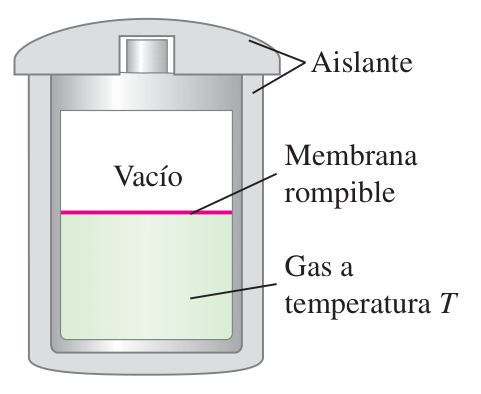
\includegraphics[width=0.5\linewidth]{imagenes/expansion-libre-gas-ideal.png}
    \caption{Gas ideal en recipiente con membrana rompible}
    \label{fig:e-int-gas-ideal}
  \end{figure}
  
  Si la membrana se rompe o se elimina, el gas se expande para llenar ambas partes del recipiente. El gas no efectúa trabajo sobre su entorno porque las paredes del recipiente no se mueven, y no fluye calor a través del aislante. Por lo tanto, $ Q $ y $ W $ son cero, y la energía interna $ U $ es constante.

  \underline{¿Cambia la temperatura durante una expansión libre?} Supongamos que sí, aunque la energía interna no lo hace. en tal caso, tendríamos que concluir que la energía interna depende de la temperatura y el volumen, o de la termperatura y la presión. Sin embargo, si $ T $ es constante durante una expansión libre, y la energía interna $ U $ se mantuvo constante a pesar de los cambios de volumen y presión, la única respuesta sería que $ U $ depende sólo de $ T $. 

  Muchos experimentos han demostrado que, cuando un gas ideal sufre una expansión libre, su temperatura \textit{no} cambia, se mantiene constante. Por lo tanto:

  \fbox{\parbox{0.9\linewidth}{
  \textbf{}
  La energía interna de un gas ideal depende sólo de su temperatura, no de su presión ni de su volumen
  }}\vspace{0.2cm}

  Aparte:

  Los gases de comportamiento no ideal suelen tener fuerzas de atracción intermoleculares y, cuando sus moléculas se separan, aumentan las energías potenciales correspondientes. Si la energía interna total es constante, las energías cinéticas deben disminuir. La temperatura está relacionada directamente con la energía cinética molecular; por lo tanto, en un gas aśi, una expansión libre usualmente va acompañada de una caída en la temperatura.

  \subsection{Capacidad calorífica del gas ideal}
  Ya habíamos hablado de la capacidad calorífica molar y que esta dependía de las condiciones en que se agrega calor. Podíamos medirla a volumen constante $ C_{V} $, o a presión constante $ C_{p} $. Pero, ¿por qué son diferentes estas dos capacidades caloríficas? Esto se debe a la primer ley de la termodinámica. Si aumenta la temperatura a volumen constante, el sistema no efectúa trabajo y el cambio de enrgía interna $ \Delta U $ es igaul al calor agregado $ Q $. En un aumento de temperatura a presión constante, en cambio, el volumen tiene que aumentar; sino la presión no podría permanecer constante. Al expandirse el material, realiza un trabajo $ W $, y como $ \Delta U = Q - W $, el suministro de calor en un proceso a presión constante debe ser mayor que en uno a volumen constante, porque se requiere energía adicional para el trabajo $ W $ realizado durante la expansión. Así, $ C_{p} $ del gas ideal es mayor que $ C_{V} $.

  \subsubsection{Relación entre las dos capacidades caloríficas para un gas ideal}
  Podemos deducir una relación sencilla entre $ C_{p} $ y $ C_{V} $ para el gas ideal. Consideremos priemro el proceso de volumen constante. Colocamos $ n $ moles de gas ideal a temperatura $ T $ en un recipiente de volumen constante, que colocamos en contacto térmico con un cuerpo más caliente; una cantidad infinitesimal de calor $ dQ $ fluye hacie el gas, y su temperatura aumenta en una cantidad infinitesimal $ dT $. Por la definición de $ C_{V} $, la capacidad calorífica molar a volumen constante,
  \[
  dQ = nC_{V}dT
  \]

  La presión aumenta durante este proceso, pero el gas no realiza trabajo ($ dW = 0 $) porque el volumen es constante. La primera ley en forma diferencial es $ dU = dQ - dW $. Como $ dW = 0 $, $ dQ = dU $ y la ecuación también la podemos escribir como 
  \[
  dU = nC_{V}dT
  \]

  Supongamos ahora un proceso a presión constante con el mismo cambio de temperatura $ dT $. Colocamos el mismo gas en un cilindro con un postón que permitimos moverse apenas lo suficiente para mantener una presión constante y ponemos el sistema en constacto con un cuerpo más caliente. Al fluir calor hacia el gas, se expande a presión constante y efectúa trabajo. Por la definición de $ C_{p} $, la cantidad de calor $ dQ $ que entra en el gas es 
  \[
    dQ = nC_{p}dT
  \]

  El trabajo $ dW $ efecutado por el gas en este proceso a presión constante es 
  \[
    dW = p\,dV
  \]

  También podemos expresar $ dW $ en términos del cambio de temperatura $ dT $ usando la ecuación de estado del gas ideal, $ pV = nRT $. Al ser $ p $ constante, el cambio en $ V $ es proporcional al cambio de $ T $:
  \[
  dW = p\,dV = nR\,dT \quad \text{Esto solo porque la presión es constante}
  \]

  Ahora sustituimos las ecuaciones que obtuvimos recién en $ dQ = dU + dW $ y nos queda:
  \[
  nC_{p}\,dT = dU + nR\,dT
  \]

  Ahora, \textbf{prestar atención}. Acá podemos meter la ecuación $ dU = nC_{V}\,dT $ que es la de volumen constante, a pesar de que ahora el volúmen no es constante. Esto lo podemos hacer porque habíamos dicho antes que, para un gas ideal, su energía interna \textit{solo depende de su temperatura}. Y si esto es válido para un proceso, tiene que ser válido para cualquier proceso con el mismo $ dT $. Por ende, podemos sustituir $ dU $ en la última ecuación que obtuvimos:
  \[
    nC_{p}\,dT = dC_{V}\,dT + nR\,dT
  \]
  Sacamos factor común $ n\,dT $ y cancelamos:
  \[
    C_{p} = C_{V} + R
  \]

  Y acabamos de demostrar que la capacidad calorífica molar del gas ideal a presión constante es mayor que a volumen constante; la diferencia es la constante de los gases ideales $ R $.

  \subsubsection{El cociente de capacidades caloríficas}
  El \textbf{cociente de capacidades caloríficas} se representa con la letra $ \gamma $ y está dado por:
  \[
  \gamma = \frac{C_{p}}{C_{V}}
  \]

  Esta capacidad desempeña un papel importante en los procesos \textit{adiabáticos} de gases ideales.

  \subsection{Proceso adiabático para el gas ideal}
  \subsubsection{Gas ideal adiabático: Relación entre V, T, y p}
  Podemos deducir una relación entre el volumen y los cambios de temperatura para un proceso adiabático infinitesimal en el gas ideal. Sabemos que, para \textit{cualquier} proceso del gas ideal tenemos $ dU = nC_{v}\,dT $. Además, el trabajo efectuado por el gas durante el proceso está dado por $ dW = p\,dV $. Entonces, dado que en un proceso adiabático $ dU = -dW $, tenemos
  \[
  nC_{V}\,dT = -p\,dV
  \]

  Para obtener una relación que solo tenga el volumen $ V $ y la temperatura $ T $, podemos sustituir $ p $ usando la ecuación del gas ideal
  \[
  nC_{V}\,dT = -\frac{nRT}{V}\,dV 
  \]
  
  Se cancela $ n $ y reordenamos
  \[
  \frac{dT}{t} + \frac{R}{C_{V}}\frac{dV}{V} = 0
  \]

  Vimos recién que podemos expresar $ R $ en función de $ C_{p} $ y $ C_{V} $, y también que $ \gamma = C_{p}/C_{V} $, entonces
  \[
    \frac{R}{C_{V}} = \frac{C_{p}-C_{V}}{C_{V}} = \frac{C_{p}}{C_{V}} - 1 = \gamma - 1
  \]

  Reemplazamos
  \[
  \frac{dT}{T} + (\gamma - 1) \frac{dV}{V} = 0
  \]

  Como $ \gamma $ siempre es mayor que 1 (porque $ C_{p} > C_{V} $, $ (\gamma - 1) $ siempre es positivo. Esto nos dice que $ dV $ y $ dT $ siempre tienen signos opuestos. Y esto tiene sentido con lo que sabemos hasta ahora ya que siempre que un gas se expande mediante un proceso adiabático, se produce una disminución de la temperatura y viceversa.

  Para cambios finitos de temperatura y volumen, integramos la ecuación:
  \begin{align*}
    \ln{T} + (\gamma - 1)\ln{V} &= \text{constante}\\
    \ln{T} + \ln{V^{\gamma - 1}} &= \text{constante}\\
    \ln{TV^{\gamma - 1}} &= \text{constante}
  \end{align*}

  y, por último, $ e $ elevado a una constante siguie siendo una constante, así que
  \[
  TV^{\gamma - 1} = \text{constante}
  \]

  Así, para un estado inicial $ (T_{1}, V_{1}) $ y un estado final $ (T_{2}, V_{2}) $, como $ \Delta U = 0 $,
  \[
  T_{1}V_{1}^{\gamma - 1} = T_{2}V_{2}^{\gamma - 1} 
  \]

  También podemos convertir la ecuación en una relación entre la presión y el volumen, eliminando $ T $ con la ayuda de la ecuación del gas ideal. Al sustituir obtenemos
  \[
  \frac{pV}{nR}V^{\gamma - 1} = \text{constante}
  \]
  
  Y como $ n $ y $ R $ son constantes, podemos hacer lo siguiente:
  \begin{align*}
    \frac{pV}{nR}\frac{V^{\gamma}}{V} &= \text{constante}\\
    pV^{\gamma} &= \text{constante}(nR)\\
    pV^{\gamma} &= \text{constante}
  \end{align*}

  Para un estado inicial $ (p_{1}, V_{1}) $ y un estado final $ (p_{2}, V_{2}) $, la ecuación se convierte en 
  \[
  p_{1}V_{1}^{\gamma} = p_{2}V_{2}^{\gamma}
  \]

  También podemos calcular el trabajo efectuado por un gas con comportamiento ideal durante un proceso adiabático. Sabemos que $ Q = 0 $ y $ W = -\Delta U $ para \textit{cualquier} proceso adiabático. Para el gas ideal, $ \Delta U = nC_{V}(T_{2} - T_{1}) $. Si conocemos el número de moles $ n $ y las temperaturas inicial y final, tenemos 
  \[
    W = nC_{V}(T_{1}-T_{2})
  \]

  También podemos usar $ pV = nRT $ en esta ecuación
  \[
    W = \frac{C_{V}}{R}(p_{1}V_{1} - p_{2}V_{2}) = \frac{1}{\gamma - 1}(p_{1}V_{1} - p_{2}V_{2})
  \]

  \section{La segunda ley de la termodinámica}
  Muchos procesos termodinámicos suceden naturalmente en una dirección pero no en la opuesta. Por ejemplo, el calor siempre fluye de un cuerpo caliente a uno más frío, nunca al revés. El flujo de calor de un cuerpo frío a uno caliente no violaría la primera ley de la termodinámica si la energía total se conserva; sin embargo, esto no ocurre. La razón de este comportamiento tiene que ver con la dirección de los procesos termodinámicos y constituye la segunda ley de la termodinámica.

  \subsection{Dirección de los procesos termodinámicos}
  Todos los procesos termodinámicos que se dan en la naturaleza son \textbf{procesos irreversibles}, es decir, procesos que se realizan en una dirección pero no en otra.

  A pesar de esto, podemos imaginar una clase de procesos idealizados que serían reversibles. Un sistema que sufre un \textbf{proceso reversible} idealizado siempre está \textit{muy cerca} del equilibrio termodinámico dentro de sí y con su entorno. Cualquier cambio de estado que se presente podría revertirse (hacer que procesa en el otro sentido). Decimos que está muy cerca porque si estuviese en equilibrio no habría cambio de estado, no habría flujo de calor, el sistema no se expandiría por lo que no realizaría trabajo sobre su entorno. Los procesos reversibles son una idealización que nunca puede lograrse en el mundo real.

  \subsection{Máquinas térmicas}
  Una \textbf{máquina térmica} es un dispositvo que transforma calor parcialmente en trabajo o energaía mecánica. Llamamos \textbf{sustancia de trabajo} a la cantidad de materia dentro de la máquina térmica que experimenta entrada y salida de calor, expansión y compresión, o cambios de fase. El tipo de máquina más fácil de analizar es aquel donde la sustancia de trabajo efectúa un \textbf{proceso cíclico}, es decir, una sucesión de procesos que al final deja la sustancia en el estado que inició.

  \subsubsection{Fuentes fría y caliente}
  Todas las máquinas térmicas absorben calor de una fuente a una temperatura relativamente alta, realizan un trabajo mecánico y desechan o rechazan algo de calor a una temperatura más baja. Si el sistema pasa por un proceso cíclico, sus energías internas inicial y final son la misma, por lo que $ Q = W $ debido a la primera ley de la termodinámica.

  En las máquinas térmicas podemos identificar dos fuentes con las cuales la sustancia de trabajo puede interactuar. Una es la \textit{fuente caliente}, que le puede dar a ala sustancia de trabajo grandes cantidades de calor a temperatura constante $ T_{H} $ sin cambiar apreciablemente su propia temperatura. La otra es la \textit{fuenta fría}, que puede absorber grandes cantidadades de calor desechado por la máquina a una temperatura constante menor $ T_{C} $.

  Las cantidades de calor transferido de las fuentes caliente y fría como $ Q_{H} $ y $ Q_{C} $ corresponden a las temperaturas $ T_{H} $ y $ T_{C} $ respectivamente.

  \subsubsection{Diagramas de flujo de energía y eficiencia}
  Podemos representar las transformaciones de energía (calor a trabajo y viceversa) en una máquina términa con el diagrama de flujo de energía de la Figura \ref{fig:diag-flujo}. 

  \begin{figure}[H]
    \centering
    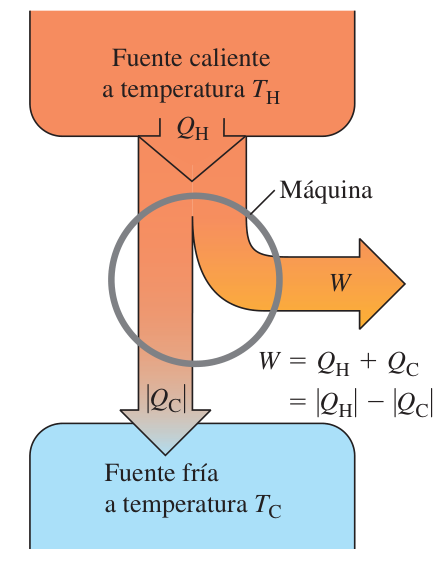
\includegraphics[width=0.5\linewidth]{imagenes/diagrama-de-flujo.png}
    \caption{Diagrama de flujo de energía para una máquina térmica}
    \label{fig:diag-flujo}
  \end{figure}
  
  La máquina en sí se representa con un círculo. La anchura de las flechas determina la cantidad de energía transferida.
  
  Si la máquina repite el mismo ciclo, $ Q_{H} $ y $ Q_{C} $ representan el calor absorbido y rechazado en un ciclo. El calor neto $ Q $ es 
  \[
    Q = Q_{H} + Q_{C} = \left|Q_{H}\right| - \left|Q_{C}\right|
  \]

  La salida útil de la máquina es el trabajo neto $ W $ que, por la primera ley, tiene que ser igual a $ Q $
  \[
    W = Q = Q_{H} + Q_{C} = \left|Q_{H}\right| - \left|Q_{C}\right|
  \]

  Idealmente, nos gustaría convertir todo el calor $ Q_{H} $ en trabajo; en tal caso, tendríamos $ Q_{H} = W $ y $ Q_{C} = 0 $, pero esto es imposible en la realidad. La \textbf{eficiencia térmica} de una máquina, denotada como $ e $, representa la cantidad de trabajo que puedo generar a partir de una cierta cantidad de calor $ Q_{H} $
  \[
  e = \frac{W}{Q_{H}} = \frac{\left|Q_{H}\right| - \left|Q_{C}\right|}{Q_{H}} = 1 - \frac{\left|Q_{C}\right|}{Q_{H}}
  \]

  \subsection{Refrigeradores}
  Los \textbf{refrigeradores} son máquinas térmicas que operan en reversa. Habíamos dicho que una máquina térmica toma calor de una lugar caliente y lo cede a un lugar más frío. Un refrigerador hace lo contrario; toma calor de un lugar mas frío y lo cede a un lugar mas caliente.

  \begin{figure}[H]
    \centering
    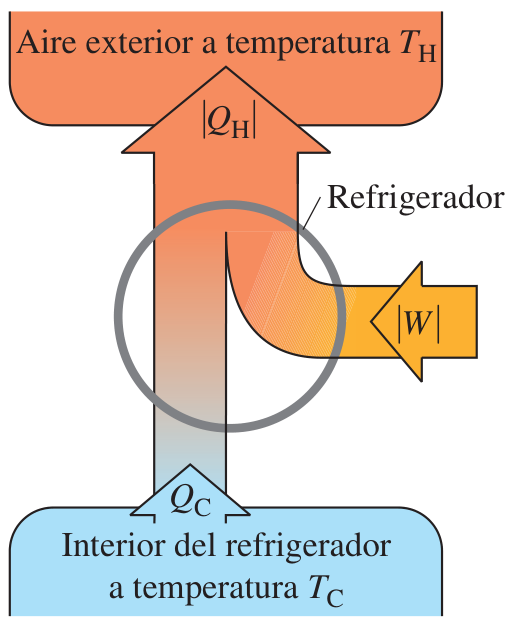
\includegraphics[width=0.4\linewidth]{imagenes/diag-flujo-refri.png}
    \caption{Diagrama de flujo de un refrigerador.}
    \label{fig:diag-flujo-refri}
  \end{figure}
  
  Vemos en la Figura \ref{fig:diag-flujo-refri} que, de acuerdo con las convenciones de signo que habíamos definido para el calor y el trabajo, $ Q_{C} $ es positivo pero $ Q_{H} $ y $ W $ son negativos en este caso.

  Al ser un proceso cíclico, por la primera ley sabemos que $ Q = W $. El calor neto es $ Q = Q_{H} + Q_{C} $. En la figura vemos que $ Q_{H} $ es mayor que $ Q_{C} $, y esto tiene sentido porque dijimos que el trabajo $ W $ en los refrigeradores era negativo.
  \[
  W = Q = Q_{H} + Q_{C} \quad  \text{o,} \quad \left|W\right| = \left|Q_{H}\right| - \left|Q_{C}\right| 
  \]

  Desde un punto de vista económico, el mejor ciclo de refrigeración es el que saca el máximo de calor $ Q_{C} $ del refrigerdador con el menor gasto de trabajo mecánico $ \left|W\right| $. Por lo tanto, la razón que nos importa es $ \left|Q_{C}\right|/\left|W\right| $; cuanto mayor sea dicha razón, mejor será el refrigerador. A esta razón se la conoce como \textbf{coeficiente de rendimiento}, y se la denota con la letra $ K $.
  \[
  K = \frac{\left|Q_{C}\right|}{\left|W\right|} = \frac{\left|Q_{C}\right|}{\left|Q_{H}\right| - \left|Q_{C}\right|}
  \]

  \subsection{La segunda ley de la termodinámica}

  \fbox{\parbox{0.9\linewidth}{
  \textbf{Segunda Ley de la Termodinámica (Kelvin-Planck)}

  Es imposible que un sistema efectúe un proceso en el que absorba calor de una fuente de temperatura uniforme y lo convierta totalmente en trabajo mecánico, terminando en el mismo estado en que inició.
  }}\vspace{0.2cm}

  Esta forma de la ley nos dice que en un proceso cíclico es imposible convertir enteramente calor en trabajo.

  \fbox{\parbox{0.9\linewidth}{
  \textbf{Segunda Ley de la Termodinámica (Clausius)}

  Es imposible que un proceso tenga como único resultado la transferencia de calor de un cuerpo más frío a uno más caliente.
  }}\vspace{0.2cm}

  Si pudieramos construir un refrigerador sin trabajo, violando este segundo planteamiento de la segunda ley, podríamos usarlo junto con una máquina térmica, bombeando el calor rechazado por la máquina de vuelta a la fuente de calor para reutilizarlo. Tendríamos energía infinita.

  \subsection{El ciclo de Carnot}
  De acuerdo con la segunda ley, ninguna máquina térmica puede tener eficiencia del 100\%. ¿Qué tanta eficiencia puede tener una máquina? La respuesta la da una máquina térmica idealizada hipotética que tiene la máxima eficiencia posible. El ciclo de esta máquina se denomina \textbf{cilco de Carnot}.


  \subsubsection{Pasos del ciclo de Carnot}
  El ciclo de Carnot es un ciclo reversible que se compone de cuatro procesos también reversibles; dos isotérmicos y dos adiabáticos.

  \begin{enumerate}[1.]
    \item El gas se expande \textbf{isotérmicamente} a temperatura $ T_{H} $, absorbiendo calor $ Q_{H} $ $ (ab) $.

    \item El gas se expande \textbf{adiabáticamente} hasta que su temperatura baja a $ T_{C} $ $ (bc) $.

    \item El gas se comprime \textbf{isotérmicamente} a $ T_{C} $, expulsando calor $ \left|Q_{C}\right| $ $ (cd) $.

    \item El gas se comprime \textbf{adiabáticamente} hasta su estado inicial a temperatura $ T_{H} $ $ (da) $.
  \end{enumerate}

  \begin{figure}[H]
    \centering
  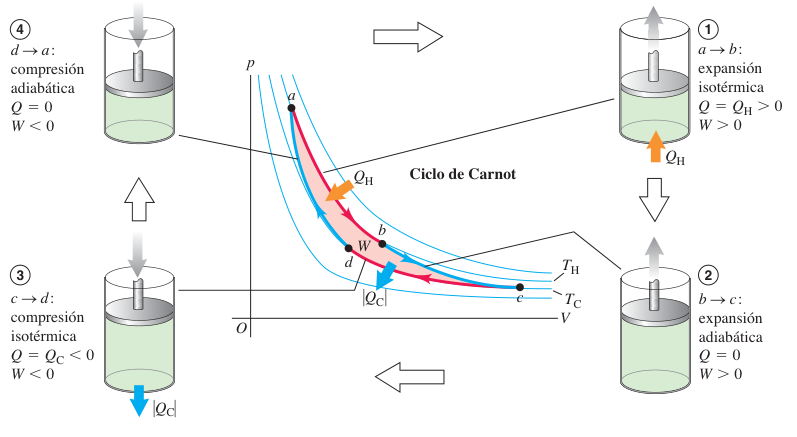
\includegraphics[width=0.8\linewidth]{imagenes/ciclo-carnot.png}
    \caption{Ciclo de Carnot para el gas ideal.}
    \label{fig:ciclo-carnot}
  \end{figure}
  
  Podemos calcular la eficiencia térmica de la máquina de Carnot cuando la sustancia de trabajo es un \textit{gas ideal}.

  La energía interna $ U $ del gas ideal depende solo de la temperatura y por ello es constante en cualquier proceso isotérmico.Para la expansión isotémrica $ ab $, $ \Delta U_{ab} = 0 $ y $ Q_{H} $ es igual al trabajo $ W_{ab} $ realizado por el gas durante su expansión isotérmica a temperatura $ T_{H} $
  \[
  Q_{H} = W_{ab} = nRT_{H}\ln{\frac{V_{b}}{V_{a}}}
  \]

  Lo mismo pasa en la expansión isotérmica $ cd $
  \[
  Q_{C} = W_{cd} = nRT_{C}\ln{\frac{V_{d}}{V_{c}}} = -nRT_{C}\ln{\frac{V_{c}}{V_{d}}}
  \]

  La razón de las dos cantidades es 
  \[
  \frac{Q_{C}}{Q_{H}} = - \left(\frac{T_{C}}{T_{H}}\right)\frac{\ln{V_{c}/V_{d}}}{\ln{V_{b}/V_{a}}}
  \]

  Podemos simplificar esta ecuación usando la relación temperatura-volumen que habíamos visto mas arriba para los procesos adiabáticos.
  \[
  T_{H}V_{b}^{\gamma - 1} = T_{C}V_{c}^{\gamma-1} \quad \text{y} \quad T_{H}V_{a}^{\gamma-1} = T_{C}V_{d}^{\gamma - 1}
  \]

  Ahora podemos dividir la primera expresión entre la segunda
  \[
  \frac{V_{b}^{\gamma-1}}{V_{a}^{\gamma-1}} = \frac{V_{c}^{\gamma-1}}{V_{d}^{\gamma-1}} \quad \text{entonces, } \quad \frac{V_{b}}{V_{a}} = \frac{V_{c}}{V_{d}}
  \]

  Esto nos dice que los dos logaritmos que habíamos visto para las ecuaciones de $ Q_{H} $ y $ Q_{C} $ son iguales, así que la ecuación del cociente entre $ Q_{C} $ y $ Q_{H} $ queda aśi:
  \[
  \frac{Q_{C}}{Q_{H}} = -\frac{T_{C}}{T_{H}} \quad \text{o} \quad \frac{\left|Q_{C}\right|}{\left|Q_{H}\right|} = \frac{T_{C}}{T_{H}} \quad \text{Transferencia de calor en la máquina de Carnot}
  \]

  Por lo tanto, la eficiencia de una máquina de Carnot es 
  \[
  e_{\text{Carnot}} = 1 - \frac{T_{C}}{T_{H}}
  \]

  \subsubsection{El refrigerador de Carnot}
  Como cada paso del ciclo de Carot es reversible,  \textit{todo el ciclo} podría revertirse, convirtiendo la máquina térmica en un refrigerador. El coeficiente de rendimiento del refrigerador de Carnot es 
  \[
  K_{\text{Carnot}} = \frac{T_{C}}{T_{H}-T_{C}}
  \]

  



  %\addcontentsline{toc}{section}{Referencias}
  %\printbibliography
  
\end{document}
